% Created 2016-02-07 Sun 17:47
\documentclass[number, sort&compress, review, 12pt]{elsarticle}
  \usepackage[utf8]{inputenc}
\usepackage{fixltx2e}
\usepackage{url}
\usepackage[version=3]{mhchem}
\usepackage{graphicx}
\usepackage{float}
\usepackage{color}
\usepackage{amsmath}
\usepackage{textcomp}
\usepackage{wasysym}
\usepackage{latexsym}
\usepackage{amssymb}
\usepackage[version=3]{mhchem}
\usepackage[linktocpage,
pdfstartview=FitH,
colorlinks,
linkcolor=blue,
anchorcolor=blue,
citecolor=blue,
filecolor=blue,
menucolor=blue,
urlcolor=blue]{hyperref}
\date{\today}
\title{manuscript}
\begin{document}

\begin{frontmatter}
\title{Core level shifts in Cu-Pd alloys as a function of bulk composition and structure}

\author[cmu]{Jacob Boes}
\author[cmu]{Peter Kondratyuk}
\author[cmu]{Chunrong Yin}
\author[cmu]{James B. Miller}
\author[cmu]{Andrew J. Gellman}
\author[cmu]{John R. Kitchin\corref{cor}}
\ead{jkitchin@andrew.cmu.edu}

\address[cmu]{Department of Chemical Engineering, Carnegie Mellon University, Pittsburgh, PA 15213}

\cortext[cor]{Corresponding author}

\begin{abstract}
CuPd alloys are important materials in hydrogen purification, where they are used as dense Pd-based separation membranes. Cu is added to impart sulfur tolerance and improved mechanical properties. At intermediate compositions and T $<$ 873 K, a BCC alloy (B2) phase occurs, which has superior separation characteristics to those of the FCC phases that form at high Cu and high Pd compositions. Identifying the composition and temperature window where the B2 phase forms is a critical need to enable the design of improved alloys. A composition spread alloy film of Cu and Pd was synthesized. The film was characterized by electron back scatter diffraction and X-ray photoelectron spectroscopy, providing the core level shifts as a function of bulk composition and bulk structure. An anomalous deviation in the Cu core level shift was observed in the composition range $0.33 < x_{Pd} < 0.55$ over which the B2 phase occurs. Density functional theory calculations were used to simulate core level shifts in the FCC and B2 alloy structures. They suggest that the anomalous deviation in core level shift is due to formation of the ordered B2 phase in this composition range.
\end{abstract}

\begin{keyword}
core level shift, composition spread alloy film, electron backscatter diffraction, density functional theory, X-ray photoemission spectroscopy, CuPd alloys, hydrogen purification
\end{keyword}
\end{frontmatter}

\section{Introduction}
\label{sec-1}
The properties of metallic alloys typically depend on alloy composition and often have regions of composition space over which they are superior to those of the pure elemental components.  Finding these regions and understanding the relationship between alloy properties and composition is a core problem of metallurgy and, more generally, the science of multicomponent materials. Very often, properties of interest are strongly dependent on alloy phase/structure, and the properties can vary dramatically across phase boundaries in composition space.

This work demonstrates a method for the experimental observation of phase boundaries in alloys based on the measurement of core level shifts (CLS) in X-ray photoemission spectroscopy (XPS) and for modeling CLSs using density functional theory (DFT). It also demonstrates a high-throughput method for mapping of CLSs with almost continuous composition resolution across large regions of alloy composition space. The ability to use XPS to identify phases makes the approach particularly useful for study of phases present in the near surface regions ($\approx$ 1-2 nm) of alloys, in thin films, and in nanoparticulate morphologies; materials whose atomistic structures may not be amenable to study by X-ray diffraction or other structural tools.

Cu$_{\text{1-}x}$Pd$_x$ alloys have been studied extensively for use as hydrogen purification membranes \cite{paglieri-2002-innov-in,kulprathipanja-2005-pd-pd,morreale-2007-exper-comput,miller-2008-surfac-segreg,obrien-2010-inhib-hydrog,peters-2011-devel-thin,martin-2013-measur-hydrog}. Pd and many of its alloys are used to separate hydrogen from gas streams because their surfaces readily dissociate \ce{H2} and because H atoms have high permeance through the Pd alloy lattice. Alloying Pd with elements such as Cu increases the mechanical strength of the membrane and also imparts tolerance to the presence of sulfur containing compounds that would otherwise poison the membrane surface. Cu$_{\text{1-}x}$Pd$_x$ alloy properties such as mechanical strength, \ce{H2} dissociation kinetics, H atom permeance, and sulfur tolerance depend on the alloy composition, $x$, and on the alloy phase structure \cite{kulprathipanja-2005-pd-pd,obrien-2010-inhib-hydrog,obrien-2011-kinet-h,obrien-2012-h-d,martin-2013-measur-hydrog}.


Cu$_{\text{1-}x}$Pd$_x$ has an interesting phase diagram. Although pure Cu and Pd both have face-centered-cubic (FCC) bulk crystal structures, Cu$_{\text{1-}x}$Pd$_x$ forms a B2 phase (body-centered-cubic (BCC), CsCl structure) at $x$ $\approx$ 0.4 and T $\le$ 873 K. Both phases are crystalline; however, the Cu and Pd atoms are ordered with respect to one another in the B2 phase but randomly distributed on the FCC lattice (see Fig. \ref{fig-struc}). The pure B2 region expands to 0.35 \textless{} $x$ \textless{} 0.46 at 700 K \cite{subramanian-1991-cu-pd-pallad}. Furthermore, some of the Cu$_{\text{1-}x}$Pd$_x$ alloy properties critical to their performance in hydrogen separation depend on the phase. For example, the solubility of H atoms in the B2 phase is roughly one-fifth that in the FCC phase \cite{martin-2013-measur-hydrog}. However, the net permeance of H atoms is almost 10\texttimes{} higher in the open lattice of the B2 phase than in the close-packed FCC lattice \cite{kamakoti-2005-predic-hydrog}. Thus, stabilizing the B2 phase to temperatures \textgreater{} 873 K would greatly improve Cu$_{\text{1-}x}$Pd$_x$ membrane performance under desired operating conditions. At the alloy surface, the kinetics of \ce{H2} dissociation are much faster on the FCC phase than on the B2 phase \cite{obrien-2011-kinet-h}. The work described herein provides a means of using high-throughput XPS measurements of Cu 2p$_{\text{3/2}}$ CLSs to map the composition region of the B2 phase as a function of temperature for Cu$_{\text{1-}x}$Pd$_x$ or ternary Cu$_{\text{1-}x\text{-}y}$Pd$_x$X$_y$ alloys.

\begin{figure}[htb]
\centering
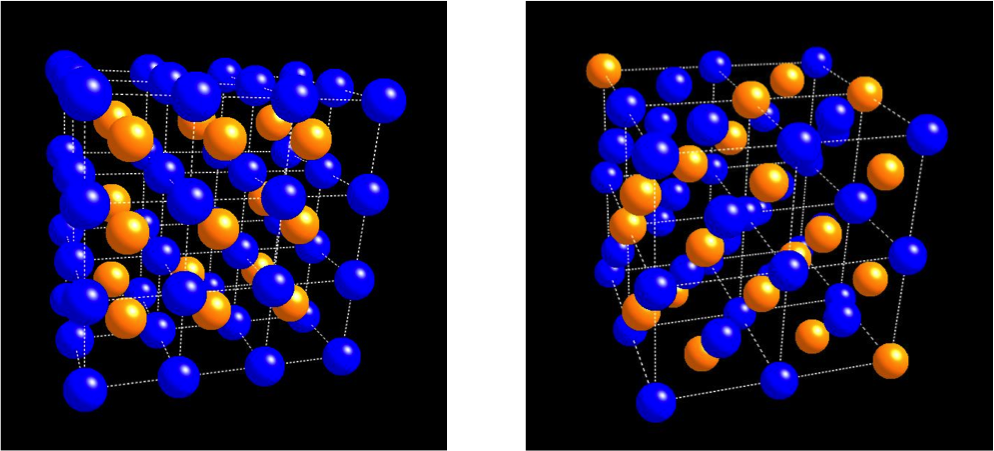
\includegraphics[width=.9\linewidth]{./images/b2-fcc.png}
\caption{.  Left. Cu$_{\text{0.5}}$Pd$_{\text{0.5}}$ ordered alloy in the B2 phase at 0 K (Pd – blue, Cu – orange).  Right. Cu$_{\text{0.3}}$Pd$_{\text{0.7}}$ disordered alloy in the FCC phase. \label{fig-struc}}
\end{figure}


Previous experimental measurements \cite{martensson-1981-elect-cu,cole-1997-deter-charg} and computed \cite{olovsson-2002-core-level} CLSs in Cu$_{\text{1-}x}$Pd$_x$ show a near linear, monotonic decrease in the Cu CLS with increasing Pd composition across the entire composition range. We observed an anomalous CLS in the composition region where the B2 phase occurs at T \textless{} 873 K. In this work, we show that the anomaly is likely due to the existence of the ordered B2 phase in this composition range. We consider the effects of configurational disorder broadening which arises from CLSs that depend on the local atomic environment of the Cu atoms \cite{marten-2005-ab-initio}. We will show that the CLS is sensitive to bulk phase ordering, and that it is possible to differentiate between the ordered B2 alloy phase and disordered FCC alloy phases using XPS.

\section{Methods}
\label{sec-2}
\subsection{Experimental}
\label{sec-2-1}
The Cu$_{\text{1-}x}$Pd$_x$ alloy samples used for XPS measurements were thin ($\approx$ 100 nm) films deposited on Mo substrates. The key experimental innovation in this work is the use of composition spread alloy films (CSAFs), deposited such that the films have continuous composition gradients lateral to their surfaces. These are high-throughput materials libraries with a continuous distribution of local compositions across a lateral dimension of $\approx$ 1 cm. The CSAFs have been deposited under ultra-high vacuum conditions using either an offset filament deposition tool or a rotating shadow mask deposition tool; both yield the same types of CSAFs and the same observations of CLSs reported in this work \cite{fleutot-2012-appar-depos,priyadarshini-2012-compac-tool}. The CSAFs have been deposited at room temperature over periods of six to eight hours and then annealed to 800 K for 1 hr to induce crystallization.

Spatially resolved XPS analysis of the Cu$_{\text{1-}x}$Pd$_x$ CSAF was conducted using a ThermoFisher ThetaProbe and yielded XP spectra from Cu$_{\text{1-}x}$Pd$_x$ alloy films spanning the entire composition space, $x$ = 0 $\rightarrow$ 1. XP spectra were obtained using a 200 $\mu$m diameter, monochromated Al K$_{\alpha}$ X-ray spot and by moving the CSAF beneath the spot to analyze regions of different composition. At each point, or alloy composition, XP spectra were obtained for the Cu 2p$_{\text{3/2}}$ and Pd 3d$_{\text{5/2}}$ lines taking 20 seconds for each element and using a 40 eV analyzer pass energy.

Prior to analysis, the films were sputtered for 6 minutes using a He$^+$ beam with an oval profile of 500 \texttimes{} 700 $\mu$m$^{\text{2}}$, a current of 4.4 $\mu$A, and a beam energy of 1 keV. This was sufficient to remove any residual O or C contamination from the surface of the film. Following sputtering, the CSAF was annealed at temperatures of 400, 500, 600, 700, and 800 K to recrystallize the near surface region damaged by He$^{\text{+}}$ sputtering.  XPS did reveal a small amount of preferential sputtering of Cu from the near surface region.  After sputtering at 300 K, this resulted in less than a 5\% change in local alloy composition relative to the composition generated by annealing at 800 K.  The alloy composition was restored to the value observed at 800 K by annealing to 600 K.  This type of behavior is consistent with prior observations of segregation in Cu$_{\text{0.3}}$Pd$_{\text{0.7}}$ alloys \cite{miller-2008-surfac-segreg}.

\subsection{Computational}
\label{sec-2-2}
All calculations were performed using the Vienna ab-initio simulation package (VASP) \cite{kresse-1993-ab,kresse-1994-ab,kresse-1996-effic,kresse-1996-effic2} with the Perdew-Burke-Ernzerhof generalized gradient approximation (GGA-PBE) \cite{perdew-1996-gener-gradien,perdew-1997-gener-gradien} exchange-correlation functional. Core electrons were described using the projector augmented wave function (PAW) \cite{blochl-1994-projec-augmen,kresse-1999-from-ultras}. \emph{k}-Points were represented using Monkhorst-Pack grids \cite{monkhorst-1976-special-point} and the Kohn-Sham orbitals were expanded up to energy cutoffs of 400 eV for all calculations. The Methfessel-Paxton scheme was used with a smearing parameter of 0.2 eV \cite{methfessel-1989-high-precis}. All calculations involving relaxations were completed with a force criteria $< 0.02$ eV/\AA{}. Ground state FCC and BCC cluster expansion calculations were performed with 3750 \emph{k}-point per reciprocal atom grids. Ground state configurations for the FCC and BCC structures of Cu$_{\text{1-}x}$Pd$_x$ were determined using a cluster expansion with ATAT \cite{walle-2002-self-monte,walle-2002-autom}. These ground state configurations identify the bulk structures of Cu and Pd that are most stable at a given bulk composition.

We used the complete screening (CS) method to compute CLSs as implemented in VASP \cite{kohler-2004-densit-funct}. This method utilizes differences in total energies of the ground and excited state of the photoemission process for a core level electron. The CLS energy \((E^{cs}_{CLS})\) is defined by the difference in chemical potential between the excited state and a reference as shown in Equation \ref{eq-cls}.

\begin{equation}
E^{cs}_{CLS} = \Delta \mu_{i} = \mu_{i} - \mu^{ref}_{i} \label{eq-cls}
\end{equation}

\noindent In this equation, the reference chemical potential is taken to be that of the pure component metal. The chemical potential of the system can then be defined as shown in Equation \ref{eq-chempot},

\begin{equation}
\mu_{i} = \frac{\partial E_{tot}}{\partial c}\biggr|_{c \rightarrow 0}  \label{eq-chempot}
\end{equation}

\noindent where \(c\) is the concentration of core-ionized atoms. Within these calculations, it is typical to remove a single electron from the core of one atom in a unit cell and place it into the valence band where it is allowed to completely screen the core-hole. Removal of a single electron simplifies the chemical potential to \(\mu_{i} = E_{ion} - E_{gs}\). Combining this difference with Equation \ref{eq-cls} we arrive at Equation \ref{eq-vasp} for the CLS of a single ion in the bulk of an alloy:

\begin{equation}
E^{cs}_{CLS}  = \left(E^{alloy}_{ion} - E^{alloy}_{gs}\right) - \left(E^{ref}_{ion} - E^{ref}_{gs}\right)  \label{eq-vasp}
\end{equation}

\section{Results and Discussion}
\label{sec-3}
\subsection{Bulk structure of the film}
\label{sec-3-1}
The bulk structure of the CSAF was determined by electron backscatter diffraction (EBSD) at points across the film. The film was annealed at 800 K prior to characterization. In EBSD, the measured diffraction pattern is compared to reference diffraction patterns to determine which structures are present. In this work, FCC and BCC structures were found. Fig. \ref{fig-phase}, shows colored images at different positions (compositions) on the film, overlaid on the phase diagram \cite{priyadarshini-2011-high-throug}. Red indicates the film in the sampled region had an FCC structure, while green indicates a BCC structure. It is evident that in the Cu and Pd rich composition ranges, the film is predominantly FCC in structure, and in the range of the known B2 phase, the film is predominantly BCC structured. In the region where mixed phases are expected, the images show mixed regions of green and red. Even though the film is thin, its phase behavior is that of a bulk alloy.

The B2 alloy phase is formally an equiatomic composition of two inter-penetrating primitive cubic lattices in the CsCl structure. As described by the phase diagram for Cu$_{\text{1-}x}$Pd$_x$ \cite{subramanian-1991-cu-pd-pallad}, the B2 phase forms at temperatures below 873 K and $x = 0.4$, shifting towards $x = 0.5$ at lower temperatures. The B2 phase is the green star that is lowest in energy shown at $x = 0.5$ in the bottom of Fig. \ref{fig-phase}. It was calculated to be stable at 0 K with respect to the FCC structures at the same composition. This is in good agreement with the phase diagram at higher temperatures and previous computational results \cite{donato-2000-bain-trans}. It is known that the composition window for the B2 phase shifts to compositions lower than $x = 0.5$ at higher temperatures \cite{bruno-2001-fermi-cu}. More recent work \cite{novikova-2014-deter-temper} at $x = 0.55$ has shown that a mixed FCC/B2 phase exists up to temperatures of 813 K, leading to some uncertainty in the literature of the exact phase boundaries for the B2 region.

Below the phase diagram in Fig. \ref{fig-phase} we show the ground state hulls for Cu$_{\text{1-}x}$Pd$_x$ alloys with FCC and BCC lattices as determined by a cluster expansion. The results are similar to previously determined ground state structures \cite{walle-2002-autom,barthlein-2007-reint-cu}. Each point on this figure represents an ordered ground state configuration for either the BCC or FCC Cu$_{\text{1-}x}$Pd$_x$ alloy. The lines connecting these points describe regions of mixed phases. The modeled configurations with the lowest formation energies are those expected at 0 K on the phase diagram. The agreement suggests that DFT is able to accurately capture the subtle energetic differences that lead to the formation of the B2 phase.

\begin{figure}[H]
\centering
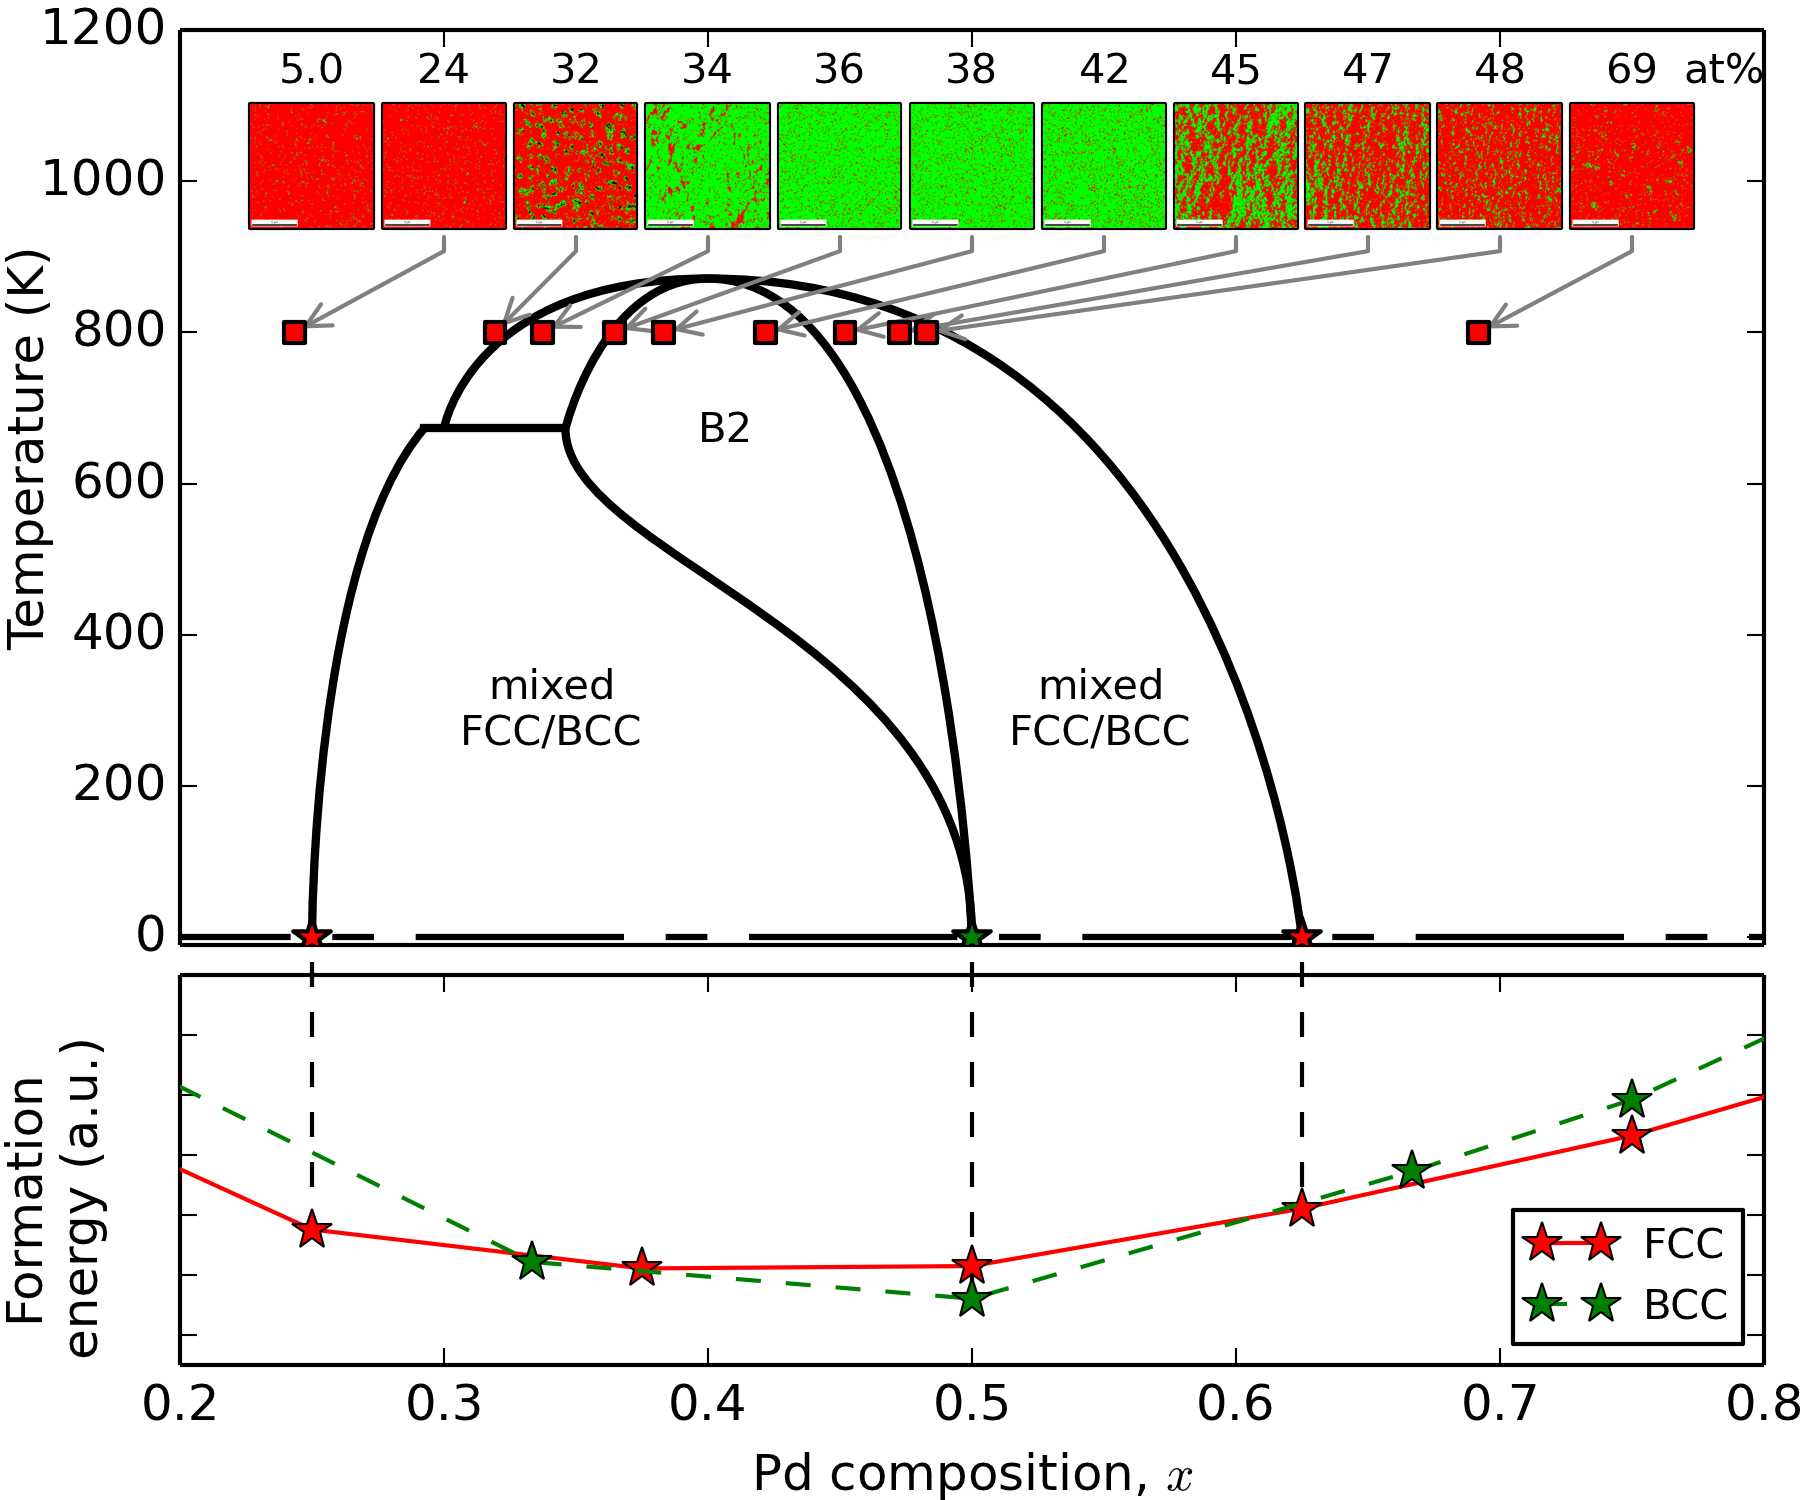
\includegraphics[width=6in]{./images/phase.png}
\caption{\label{fig-phase}In the top of the figure, electron backscatter phase maps are overlaid on a phase diagram showing the FCC (red) and BCC (green) phase behavior of the CSAF at different compositions \cite{subramanian-1991-cu-pd-pallad}. The BCC phases coincide with the known B2 range of the phase diagram at 800 K. In the bottom of the figure are ground state computational structures (stars) compared with their corresponding position on the phase diagram.}
\end{figure}

\subsection{Experimental alloy core level shifts}
\label{sec-3-2}
We measured the Cu 2p$_{\text{3/2}}$ CLSs of the alloy across the composition space of the film using XPS (Fig. \ref{fig-lit}). At the Cu-rich side, the Cu CLS decreases linearly with increasing Pd composition until about $x = 0.35$. At this point, an anomalous deviation in the CLS is observed, which continues until $x = 0.56$, where the initial linear, monotonic trend appears to resume. The onset of the anomalous CLS coincides approximately with the initial appearance of the Cu-rich  mixed FCC/B2 range, continues through the B2 region, through the high Pd mixed phase region and ends at the FCC, Pd-rich region. The monotonic trends in the FCC regions are consistent with previous literature reports (also shown in Fig. \ref{fig-lit}) \cite{cole-1997-deter-charg,martensson-1981-elect-cu}. However, the anomalous deviation in the CLS at the compositions of the B2 phase has not been reported before to our knowledge. Neither previous report mentions the annealing temperature, and it is possible that the alloy samples were annealed to temperatures where only the FCC solid solution exists across the entire composition range. We hypothesize that the anomaly in this work is due to the coexistence of the B2 phase in this region, because at the annealing temperature of 800 K, the B2 phase is expected to be stable for compositions in the range of $x=0.35-0.55$.

\begin{figure}[H]
\centering
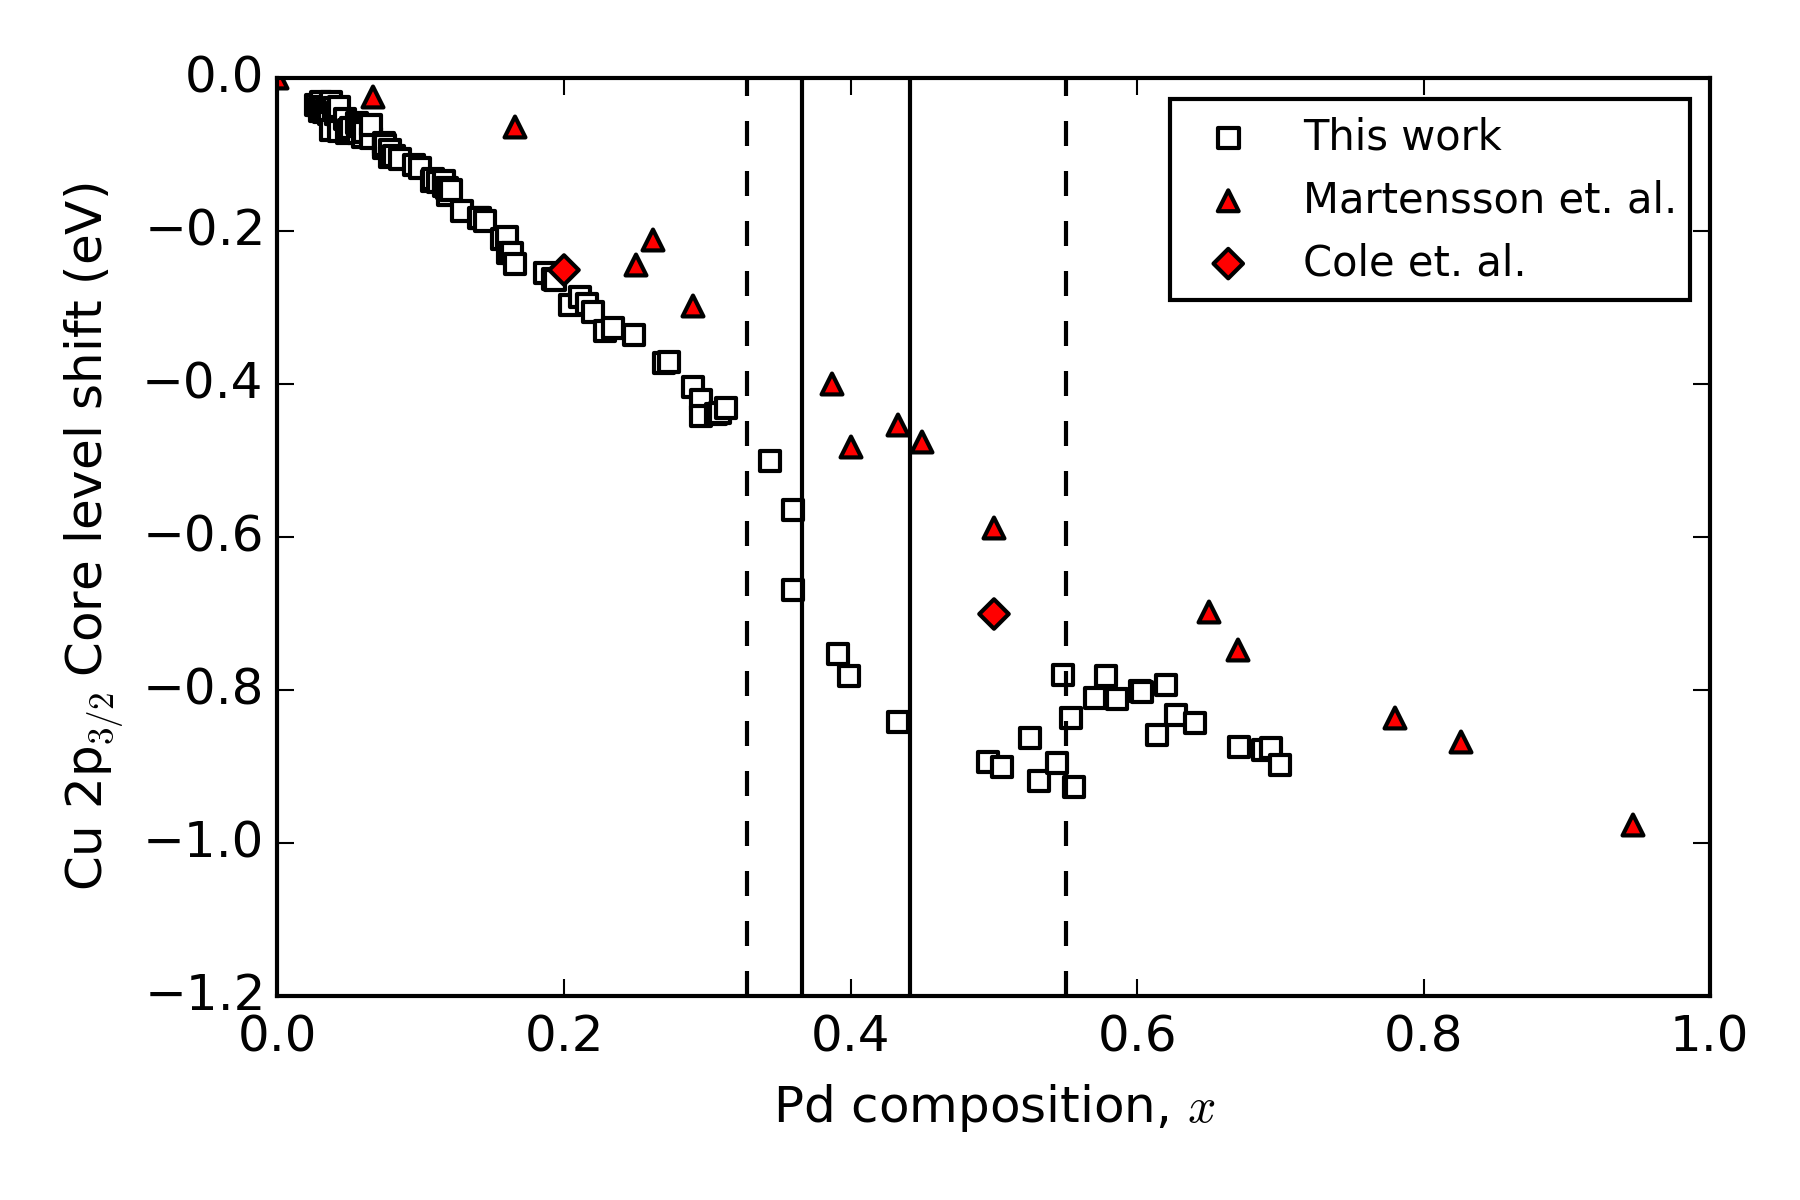
\includegraphics[width=6in]{./images/experiment.png}
\caption{\label{fig-lit}Experimentally measured bulk composition dependent Cu CLS (this work, open squares) compared to previous experimental results (red triangles \cite{martensson-1981-elect-cu}, red diamonds \cite{cole-1997-deter-charg}). The solid vertical lines delineate the B2 region, and the dashed lines delineate the mixed region boundaries at 800 K in the experimental phase diagram.}
\end{figure}

The discontinuous CLS at compositions near those of the B2 phase suggests that the origin of the discontinuity is associated with the transition from the close-packed FCC solid solution to the more open BCC lattice of the B2 phase. Additional evidence for this comes from XPS study of the CSAF following He$^{\text{+}}$ ion sputtering. Fig. \ref{fig-sputtering} shows the Cu 2p$_{\text{3/2}}$ CLS versus Cu$_{\text{1-}x}$Pd$_x$ composition as measured on a CSAF deposited using the rotating shadow mask CSAF deposition tool \cite{fleutot-2012-appar-depos}.  The CSAF preparation includes annealing at 800 K for 1 hr prior to removal from the deposition chamber. This as-prepared CSAF exhibits the Cu 2p$_{\text{3/2}}$ CLS behavior (not shown) associated with the B2 phase (Fig. \ref{fig-sputtering}). Sputtering of the CSAF with He$^+$ at 1 keV causes sufficient damage to the near surface region that the FCC-B2-FCC transition is no longer observed in the CLS measurements (Fig. \ref{fig-sputtering}, solid red squares). Sputter-induced alloying has previously been observed in Cu$_{\text{1-}x}$Pd$_x$ films supported on Mo single crystals \cite{rainer-1995-core-level}. However, after annealing the CSAF in vacuum at 800 K for 1 hr the anomalous CLS (open squares) associated with the B2 phase reappears. In fact, the B2 phase appears to be fully formed after annealing at only 600 K for 1 hr.

\begin{figure}[H]
\centering
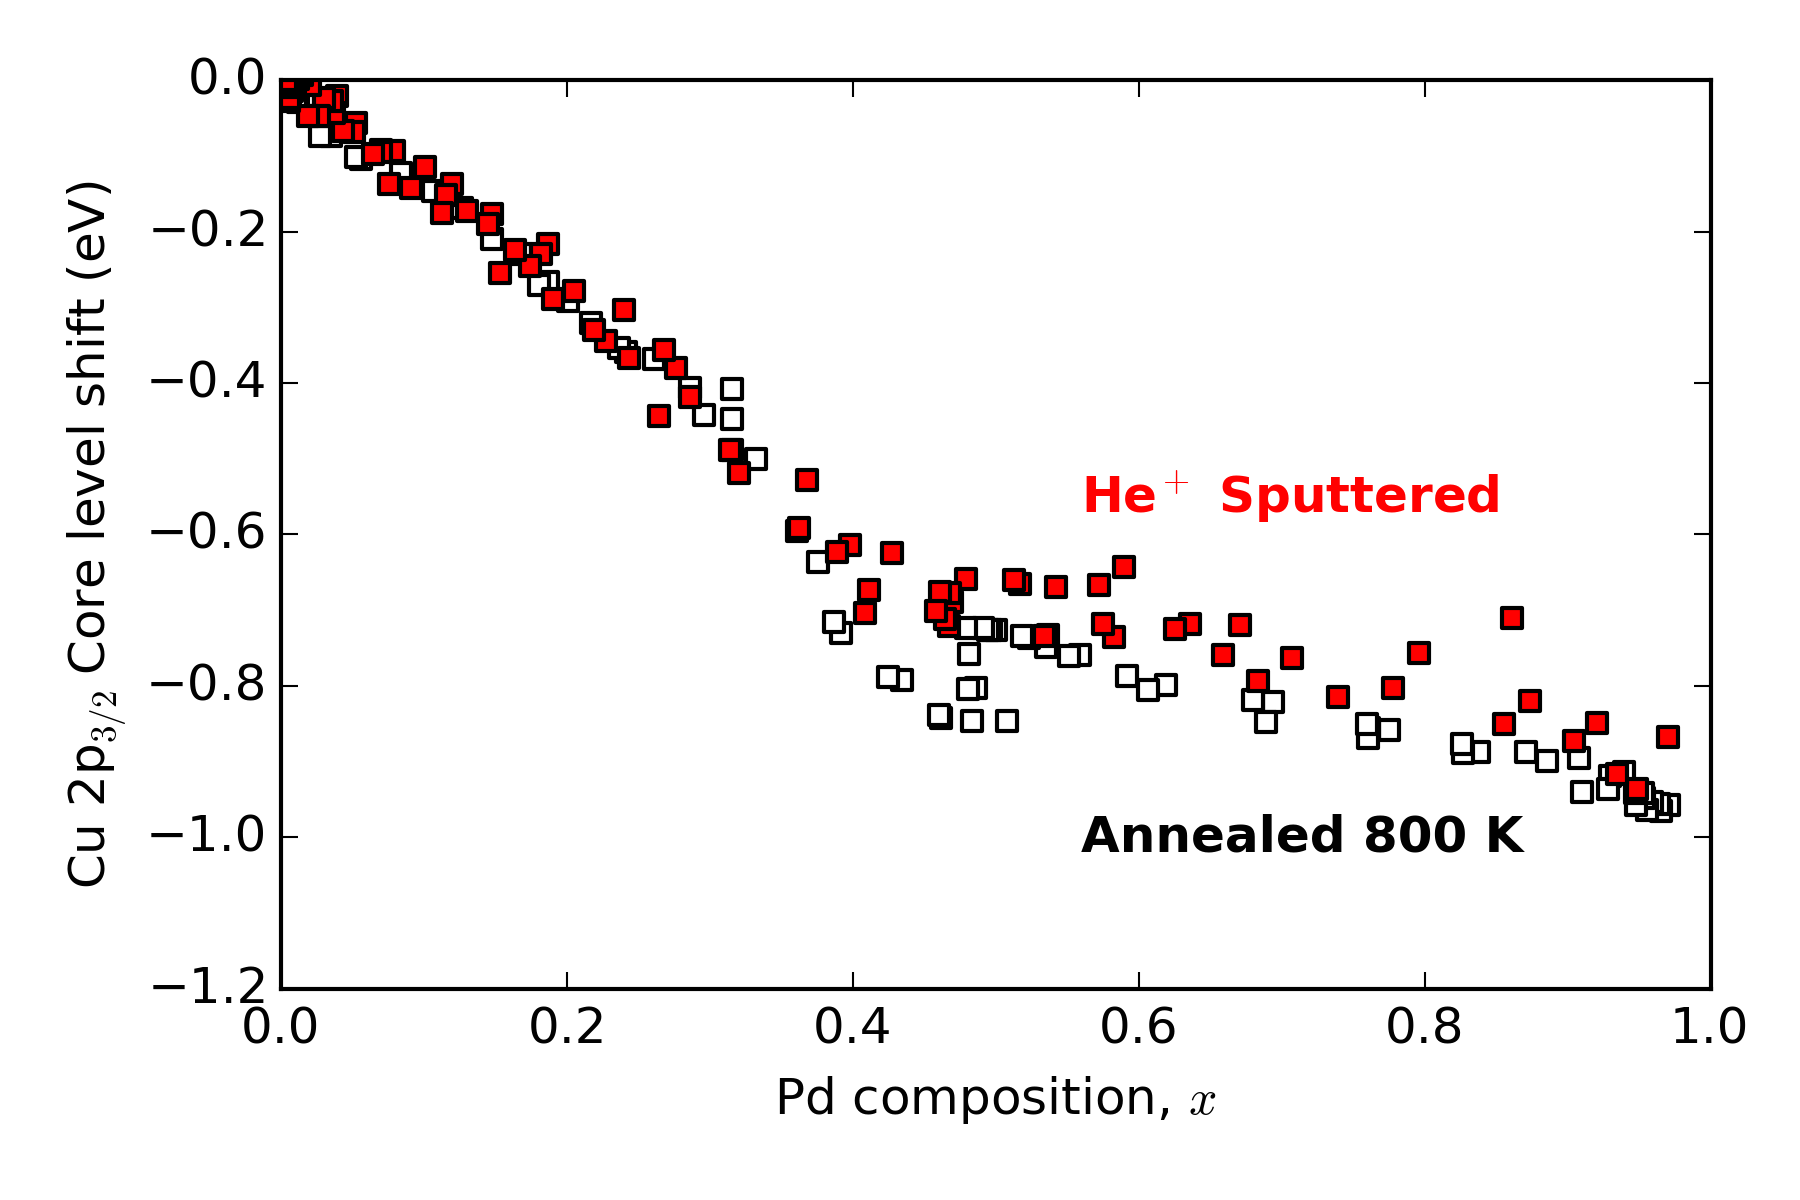
\includegraphics[width=6in]{./images/sputtering.png}
\caption{\label{fig-sputtering}Cu 2p$_{\text{3/2}}$ CLS versus Cu$_{\text{1-}x}$Pd$_x$ composition. The Cu 2p$_{\text{3/2}}$CLS measured after He$^{\text{+}}$ ion sputtering at 1 keV for six minutes (solid red squares) show a clear suppression of the CLS associated with the B2 phase. This B2-related CLS reappears after annealing at 800 K for 60 minutes (open squares).}
\end{figure}

\subsection{Computational alloy core level shifts}
\label{sec-3-3}
To test the hypothesis that the anomalous CLS could be due to the (co)existence of the B2 phase, we calculated the Cu CLS for an ordered, groundstate FCC Cu$_{\text{1-}x}$Pd$_x$ alloy at $x = 0.5$, and for the stoichiometric B2 phase. These two structures have nearly identical CLS near -1.1 eV, and neither result agrees well with the experimentally observed CLS at this composition which is near -0.9 eV.

The random FCC alloy has Cu atoms in an inhomogeneous distribution of local environments that could affect the Cu CLS \cite{marten-2005-ab-initio}. In contrast, the ordered FCC structure has a homogeneous distribution of local environments. To determine the effect of disorder on the CLS, we constructed a 64 atom FCC bulk supercell, and randomly populated the sites with 32 Cu and 32 Pd atoms. We then calculated the Cu 2p$_{\text{3/2}}$ CLS of each Cu atom. The distribution of the Cu CLSs is illustrated in Fig. \ref{fig-result} as a bar and whisker plot. The mean of this distribution is an estimation of the expected CLS for a random FCC alloy. This distribution is consistent with previously reported computational CLSs of a random Cu$_{\text{0.5}}$Pd$_{\text{0.5}}$ alloy \cite{olovsson-2006-core-level}. In the whisker plot, the bottom and top of the box represent the first and third quartiles of the distribution, the bar in the middle represents the median of the data, and the dashed error bars represent the upper and lower limits of the data; data points outside those limits can be considered outliers. The distribution average lies approximately on the center of the experimental data at $x = 0.5$. It is evident from these results that configurational disorder increases the average CLS. Next, we show that this is primarily due to the average number of Cu-Cu nearest-neighbors in the structure.

\begin{figure}[H]
\centering
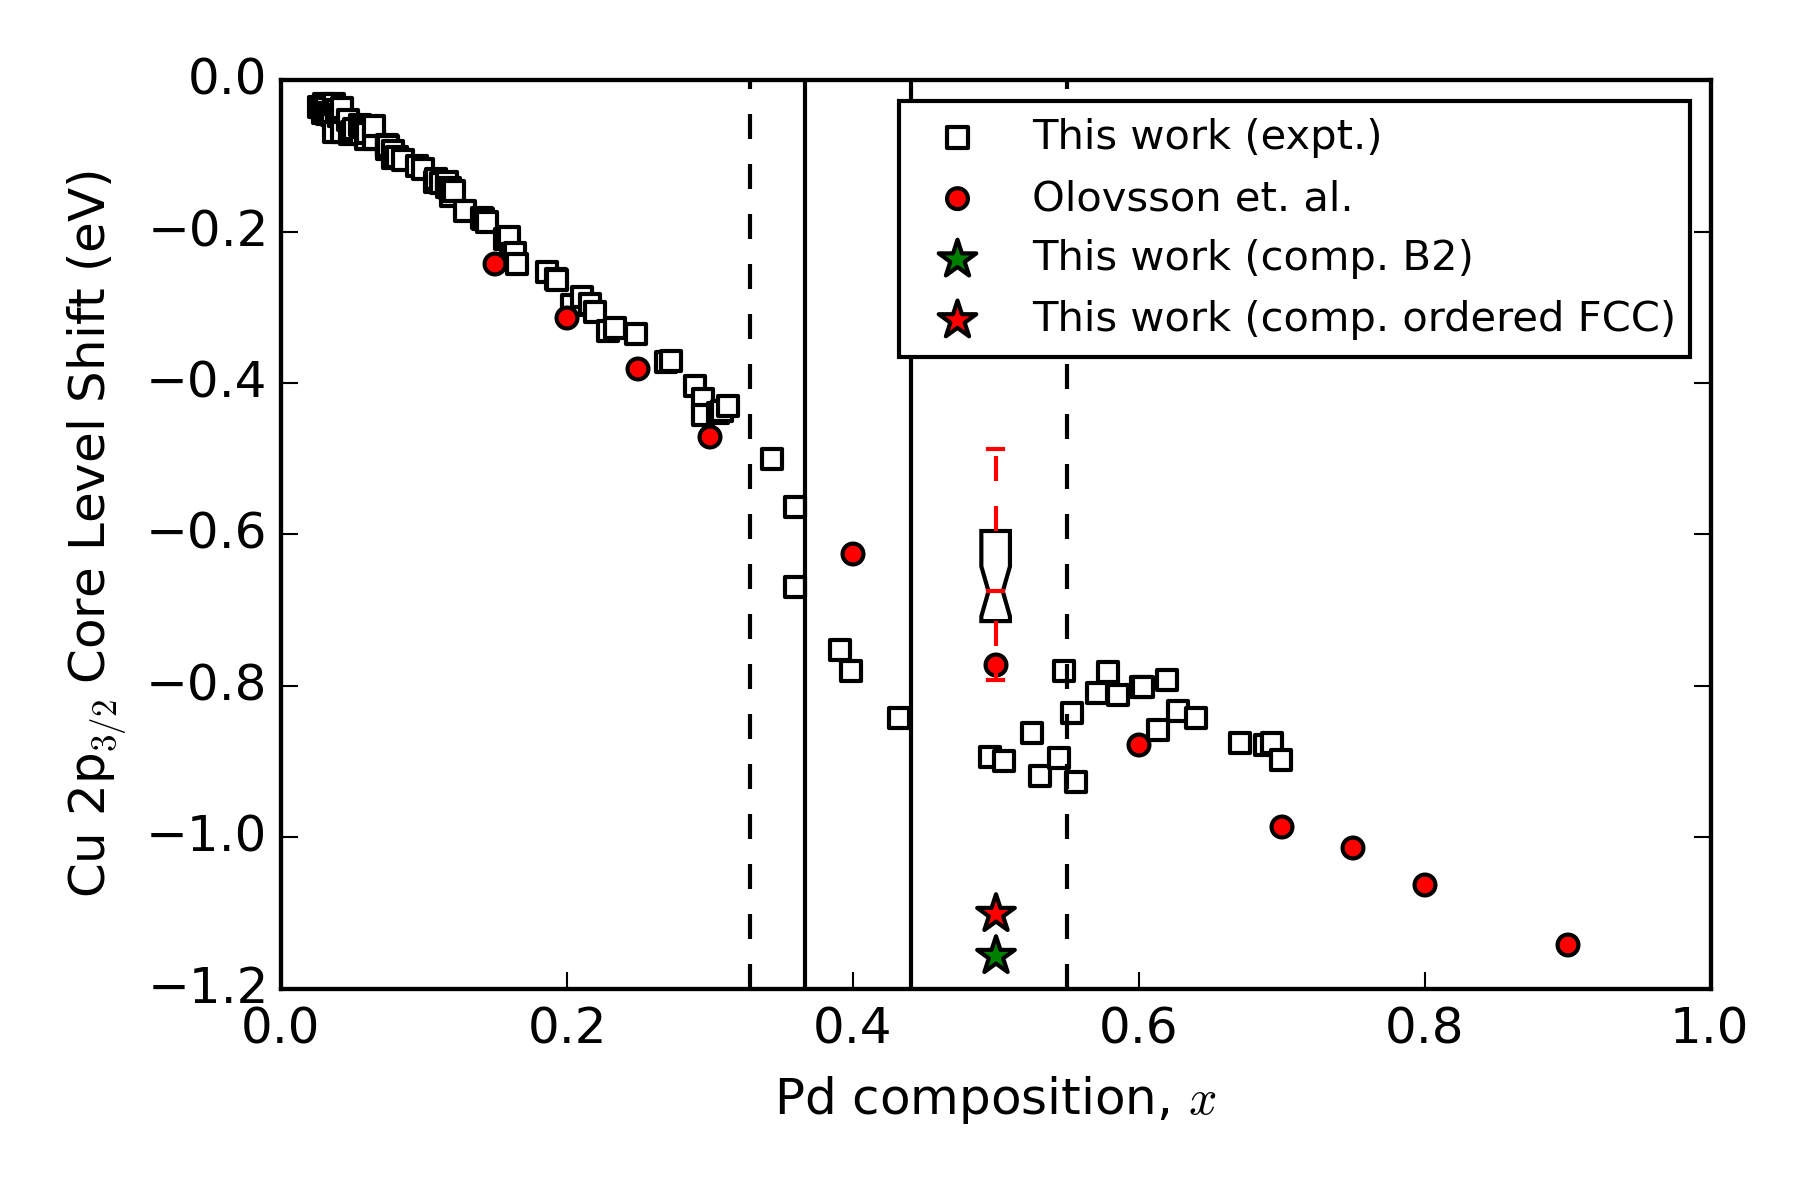
\includegraphics[width=6in]{./images/result.png}
\caption{\label{fig-result}Comparison of peak widening and ground state CLS calculations with the experimental data (open squares) for Cu CLS in Cu$_{\text{1-}x}$Pd$_x$ alloy. Computational work \cite{olovsson-2002-core-level} shown in red for randomly configured FCC alloy (circles), for ordered FCC structure (this work, red star) and B2 structure (green star). The bar and whisker plot shows the calculated (this work) distribution of the Cu CLS in a randomly ordered FCC alloy.}
\end{figure}

The primary difference between the ordered and disordered phases is that in the ordered phase, the local environments are homogeneous, whereas, in the disordered phase, there is an inhomogeneous distribution of local environments. We define the local environments by the number of nearest-neighbor Cu-Cu atoms. In Fig. \ref{fig-cls-nimp} we show that the CLS changes approximately linearly with the number of Cu-Cu nearest-neighbor atoms. The disordered FCC lattice is likely to have more Cu-Cu nearest-neighbor atom pairs, and hence a less negative average CLS than the ordered FCC structure. Due to the relatively high annealing temperature, it is unlikely that the ordered FCC phase can exist, and we do not believe it contributes significantly to the experimental observations. The B2 phase, however, is expected to be ordered at the temperatures used in this work, and consequently the Cu atoms will have fewer nearest-neighbor Cu atoms than in the FCC solid solution. As a result the B2 phase will have a  more negative CLS than the disordered FCC phase.

\begin{figure}[H]
\centering
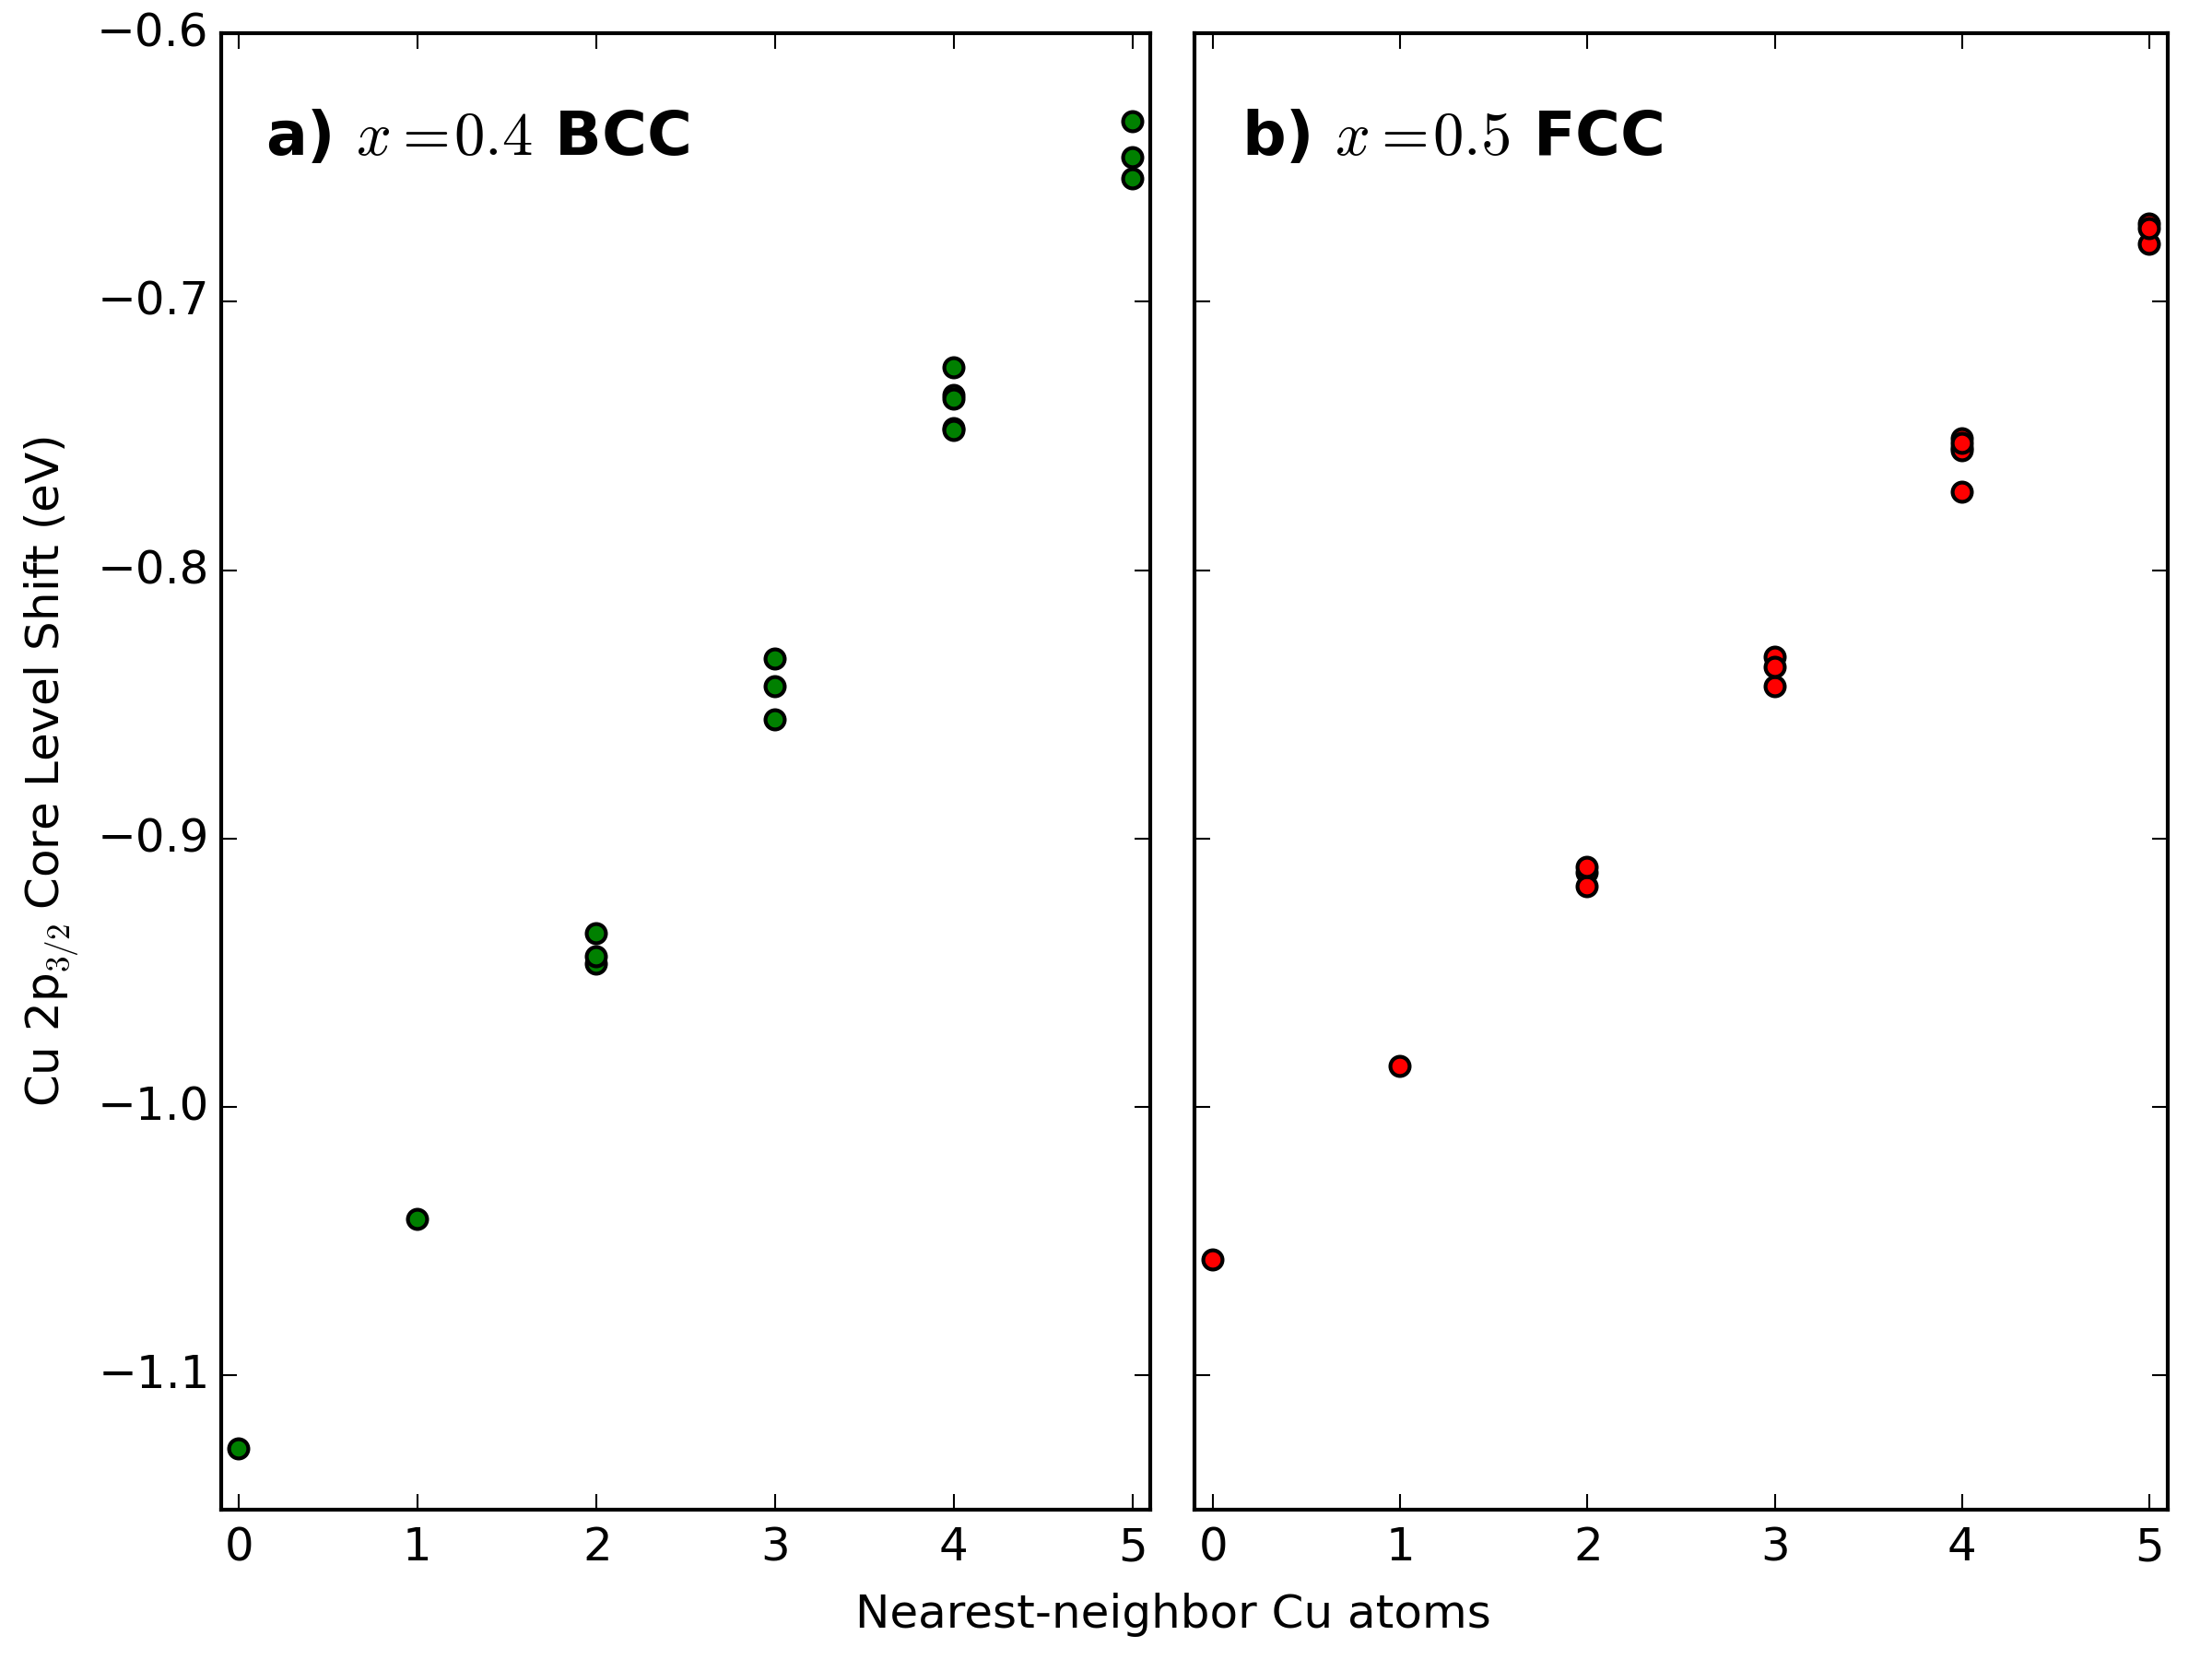
\includegraphics[width=6in]{./images/impurity.png}
\caption{\label{fig-cls-nimp}Effect of the number of nearest-neighbor Cu atoms on the calculated CLS of a Cu atom in a) the B2 structure at a lattice constant consistent with 40\% Pd and with different numbers of Cu atom nearest neighbors and b) in the ordered FCC structure at $x=0.5$ with different numbers of nearest neighbor Cu atoms. There are multiple points for each nearest-neighbor number because there are different local environments.}
\end{figure}

The calculated Cu CLS for the B2 phase was performed at the stoichiometric B2 composition ($x = 0.5$), which falls in the mixed phase region of the phase diagram at the film annealing temperature. This composition will have some B2 and some FCC phase, and the measured CLS is likely to be an average of the two phases. We next consider the impact on the B2 CLS of non-stoichiometric compositions in the experimental B2 region. The deviation from $x = 0.5$ requires that there be substitutions of Cu for Pd on the Pd sublattice, which leads to an increase in the number of Cu-Cu nearest-neighbors.

We next consider the effect of changing the alloy composition from stoichiometric $x = 0.5$ in the B2 phase to $x = 0.4$. It is not simple to model the B2 phase exactly at this composition, so we make the following approximations. First, the non-stoichiometry must be accommodated on the Pd sublattice. Second, we note that the CLS of an atom depends primarily on the distance of the nearest-neighbors (determined by the overall lattice constant), and the identity of the nearest-neighbors. We found that the identity of atoms further away than the nearest-neighbors had very little effect on the CLS. Third, the BCC Cu$_{\text{1-}x}$Pd$_x$ alloy approximately follows Vegard's law, which enables us to predict a lattice constant of the B2 phase at $x = 0.4$. Full details supporting these approximations can be found in the supporting information. Thus, there are two influences on the CLS of a Cu atom in the B2 phase: 1) the Cu atom will be in an alloy with a smaller lattice constant than the stoichiometric B2 phase, and 2) the Cu atom will have more Cu nearest-neighbors than the stoichiometric B2 alloy.

We first consider the effect of strain. As the amount of Cu in the alloy increases, the average lattice constant will decrease because Cu is a smaller atom than Pd. Fig. \ref{fig-clsvol} shows that this decreases the magnitude of the calculated CLS. The addition of Cu atoms on the Pd sublattice will also decrease the magnitude of the CLS, as seen in Fig. \ref{fig-cls-nimp}. The combined effect is consistent with the results in Fig. \ref{fig-result} which shows the magnitude of the CLS decreasing with increasing Cu.

\begin{figure}[H]
\centering
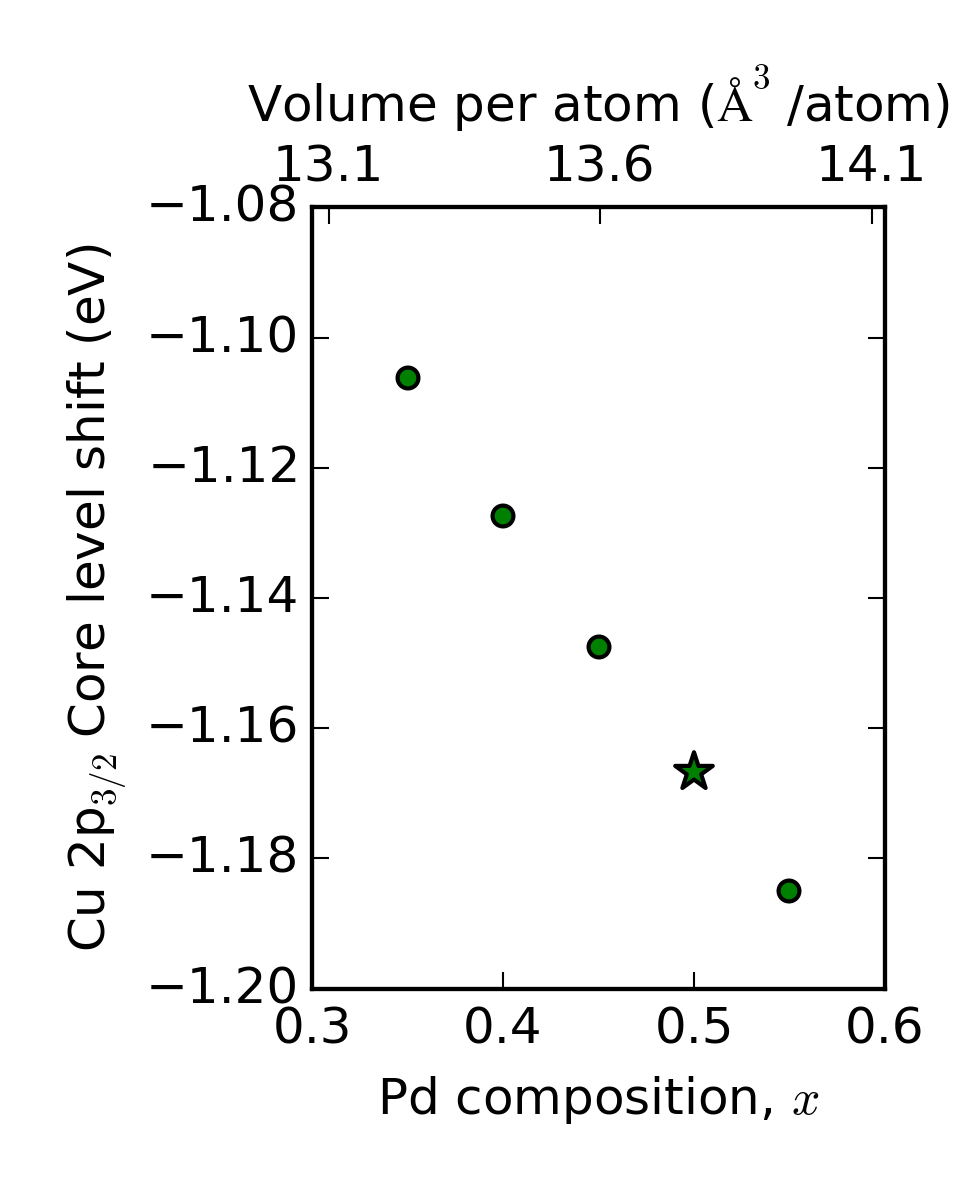
\includegraphics[width=3in]{./images/strain.png}
\caption{\label{fig-clsvol}Effects of lattice constant on the calculated CLS of the ordered B2 phase. The star represents the CLS of the stoichiometric B2 phase at the ground state volume.}
\end{figure}

Putting these results all together, we have cluster expansion and experimental EBSD results (Fig. \ref{fig-phase}) that show that the bulk alloy film has a BCC structure in the range of $0.36 < x < 0.42$, with a mixed phase region on each side of that range. The computational results show that the CLS for the B2 structure at $x = 0.5$ is considerably more negative than the corresponding disordered FCC alloy at the same composition. Additional Cu in the B2 phase is accommodated on the Pd sublattice, and simultaneously decreases the lattice constant, while increasing the average number of nearest-neighbor Cu atoms, both of which cause the CLS to become more negative. The sum of these results suggests strongly that the anomalous CLS observed in the experiments is due to the presence of a nonstoichiometric, partially ordered B2 phase in that composition region.

\section{Conclusions}
\label{sec-4}
On the Cu$_{\text{1-}x}$Pd$_x$ phase diagram at 800 K, there is a region between $0.33 < x < 0.55$ where an ordered B2 or mixed B2/FCC solid solution phase exists. Experimental CLS measurements of CSAF surfaces annealed to 800 K were compared with previously measured CLSs of randomly ordered FCC Cu$_{\text{1-}x}$Pd$_x$. From the CSAF results, an anomalous downward deviation in the CLS was observed at the composition range associated with the B2 phase at 800 K. The anomaly disappears upon sputtering the surface, and reappears on annealing.

We used density functional theory to compute the CLS of both randomly configured and ordered alloy structures in the FCC and BCC lattices. The calculated CLS of the B2 phase lies well below the CLS predicted by computations for the randomly ordered FCC phase. Nonstoichiometry in the B2 phase was accounted for by determining the effect of the lattice constant on the CLS, and the effects of nearest-neighbor Cu atoms on the CLS. Both effects decrease the magnitude of the CLS, consistent with the experimentally observed results. This suggested that the anomaly in the experimental CLS can be explained by the presence of the ordered B2 phase.

\section*{Acknowledgement}
JRK gratefully acknowledges partial support from the DOE Office of Science Early Career Research program (DE-SC0004031). AJG gratefully acknowledges support from the NSF under grant number CBET-0923083. NSF grant
CBET-923083 is acknowledged for support of the development of the RSM-CSF
deposition apparatus used in the course of this work.

\bibliographystyle{elsarticle-num}
\bibliography{/Users/jkitchin/Desktop/cappa/kitchingroup-51/manuscript}
% Emacs 25.1.50.1 (Org mode 8.2.10)
\end{document}